\documentclass[11pt]{article}

\usepackage[margin=1in]{geometry}
\usepackage[T1]{fontenc}
\usepackage{lmodern}
\usepackage{microtype}
\usepackage{amsmath,amssymb}
\usepackage{booktabs}
\usepackage{graphicx}
\usepackage{xcolor}
\usepackage[numbers,sort&compress]{natbib}
\usepackage{tikz}
\usetikzlibrary{positioning,arrows.meta,fit,calc}
\usepackage[colorlinks=true,linkcolor=blue!60!black,citecolor=blue!60!black,urlcolor=blue!60!black]{hyperref}
\usepackage{cleveref}

\newcommand{\tok}[1]{\texttt{<#1>}}

\title{\textbf{Hale-VLM: Registry-Driven, Parameter-Efficient Vision--Language Models\\on Dense Reasoning LLMs, with SmolVLM and SmolVLA Data Pipelines}}
\author{B A NaveenKumar\\
\small Independent researcher\\
\small \url{https://github.com/basaanithanaveenkumar/Hale-VLM}}
\date{}

\begin{document}
\maketitle

\begin{abstract}
Turning a strong text-only LLM into a vision--language model (VLM) is conceptually simple:
connect a pretrained image encoder through a small projector and fine-tune. In practice,
most effort goes into the surrounding system: which parameters to train, how to express
multi-stage data mixtures reproducibly, how to stream tens of large datasets without
exhausting disk, and how to reuse robotics data. We present \textbf{Hale-VLM}, an
open framework that builds VLMs on 7--8B dense reasoning LLMs (Qwen3-8B and
DeepSeek-R1-Distill-Qwen-7B) from a frozen SigLIP encoder, a trainable MLP projector and
LoRA adapters. The frozen parts stay frozen, and only $\approx$72--84M parameters (about 1\%
of the model) are updated. Every component is a plugin in the HaleBlocks registries
(models, losses, trainers, datasets), so a whole experiment, including backbone,
trainability policy and data mixture, is one inheritable YAML file. The framework ships a
typed registry of all 19 datasets of the SmolVLM training recipe, grouped by stage
(vision, video, long context), with a disabled entry documenting the recipe's rejected
data. It also ships a registry of the SmolVLA robotics corpus (534 community datasets,
simulation and real-world sets) and a converter that turns robot frames into VLM samples
for pretraining, fine-tuning or instruction tuning. A sequential streaming mixer prefetches
the next dataset while the current one is consumed, which bounds local storage. We
describe the design, give exact trainable-parameter budgets, and report two input-pipeline
issues we found in the current release, so that results built on it can be interpreted
correctly.
\end{abstract}

\section{Introduction}

The LLaVA family~\cite{liu2023llava,liu2024llava15} established a simple, strong VLM
recipe: a pretrained vision encoder, an MLP projector and an LLM, trained on
instruction-formatted image--text data. Later work showed that the \emph{data} matters at
least as much as the architecture. Idefics2~\cite{laurencon2024matters} studied design
choices and mixtures, and SmolVLM~\cite{marafioti2025smolvlm} published a detailed
multi-stage recipe with explicit ablations, including data that \emph{hurt} and was
removed. At the same time, reasoning-tuned dense LLMs such as Qwen3~\cite{qwen3} and
DeepSeek-R1 distillations~\cite{deepseekr1} have become attractive language backbones.

Hale-VLM packages these ingredients into a framework designed for controlled
experimentation:
\begin{itemize}
  \item \textbf{Parameter-efficient by default.} SigLIP~\cite{zhai2023siglip} and the LLM
        stay frozen. A two-layer MLP projector and LoRA~\cite{hu2022lora} adapters on all
        attention and MLP projections are trained, and a dedicated trainer hands the
        optimiser only these parameters (\cref{sec:model}).
  \item \textbf{Registry-driven experiments.} Model variants, losses, the trainer and
        datasets are registered plugins of HaleBlocks~\cite{haleblocks}, and experiments are
        inheritable YAML files validated by typed schemas (\cref{sec:framework}).
  \item \textbf{Reproducible data recipes.} A typed catalog of the SmolVLM stages and the
        SmolVLA~\cite{shukor2025smolvla} robotics corpus, a bounded-storage streaming
        mixer, and a robotics-to-VLM converter (\cref{sec:data}).
\end{itemize}

\section{Related Work}

\paragraph{Connecting vision encoders to LLMs.} Flamingo~\cite{alayrac2022flamingo} inserts
gated cross-attention into a frozen LLM. BLIP-2~\cite{li2023blip2} learns a Q-Former
bottleneck between frozen models. LLaVA~\cite{liu2023llava,liu2024llava15} shows that an MLP
projector over patch features, placed in the token sequence, is sufficient.
LLaVA-OneVision~\cite{li2024llavaonevision} extends this to single-image, multi-image and
video tasks. Hale-VLM follows the projector design and keeps both towers frozen, adapting
the LLM with LoRA~\cite{hu2022lora}.

\paragraph{Data recipes.} SmolVLM~\cite{marafioti2025smolvlm} trains in stages: a vision stage
based on the Cauldron mixture~\cite{laurencon2024matters} with document, OCR and
handwritten-math data, a video stage mixing descriptions, temporal understanding,
narrative, multi-image and a share of text SFT, and a long-context extension on text
corpora. It reports that reusing LLM-SFT data (SmolTalk) hurt both video and image
performance. SmolVLA~\cite{shukor2025smolvla} trains a compact VLA on hundreds of
community-contributed LeRobot datasets. Hale-VLM encodes both recipes as registries.

\section{Model}
\label{sec:model}

\begin{figure}[t]
\centering
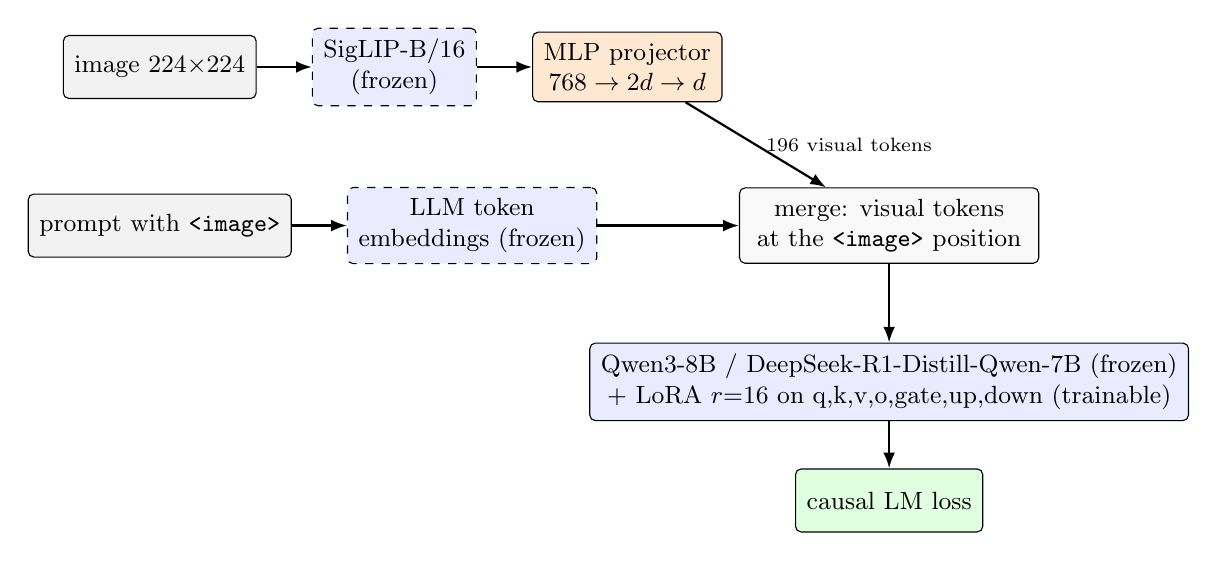
\begin{tikzpicture}[
  node distance=5mm and 7mm,
  box/.style={draw, rounded corners=2pt, align=center, font=\small, minimum height=8mm, inner sep=4pt},
  frozen/.style={box, fill=blue!8, dashed},
  train/.style={box, fill=orange!18},
  arr/.style={-{Latex[length=2mm]}, thick}
]
\node[box, fill=gray!10] (img) {image $224{\times}224$};
\node[frozen, right=of img] (sig) {SigLIP-B/16\\(frozen)};
\node[train, right=of sig] (proj) {MLP projector\\$768\to2d\to d$};
\node[box, fill=gray!10, below=12mm of img] (txt) {prompt with \tok{image}};
\node[frozen, right=of txt] (emb) {LLM token\\embeddings (frozen)};
\node[box, fill=gray!5, right=18mm of emb, minimum width=38mm] (merge) {merge: visual tokens\\at the \tok{image} position};
\node[box, fill=blue!8, below=10mm of merge, minimum width=62mm] (llm) {Qwen3-8B / DeepSeek-R1-Distill-Qwen-7B (frozen)\\+ LoRA $r{=}16$ on q,k,v,o,gate,up,down (trainable)};
\node[box, fill=green!12, below=6mm of llm] (loss) {causal LM loss};
\draw[arr] (img) -- (sig); \draw[arr] (sig) -- (proj);
\draw[arr] (txt) -- (emb); \draw[arr] (emb) -- (merge);
\draw[arr] (proj) -- node[right, font=\scriptsize]{196 visual tokens} (merge);
\draw[arr] (merge) -- (llm); \draw[arr] (llm) -- (loss);
\end{tikzpicture}
\caption{Hale-VLM. Dashed boxes are frozen and orange boxes are trained. The LLM is frozen
except for its LoRA adapters.}
\label{fig:arch}
\end{figure}

\paragraph{Vision tower and projector.} Images are resized to $224\times224$ and encoded by
SigLIP-B/16~\cite{zhai2023siglip} (CLIP~\cite{radford2021clip} is also supported), producing
196 patch features of width 768. A projector maps them into the LLM embedding space,
either linearly or with an MLP $768\to 2d\to d$ with GELU, where $d$ is the LLM hidden size.
At most \texttt{num\_image\_tokens} projected tokens are kept.

\paragraph{Language backbone.} Two dense backbones are supported through
\texttt{transformers}. Qwen3-8B~\cite{qwen3} (36 layers, $d=4096$, FFN 12{,}288, grouped-query
attention with 32 query and 8 key--value heads of width 128) is the default.
DeepSeek-R1-Distill-Qwen-7B~\cite{deepseekr1} (28 layers, $d=3584$, FFN 18{,}944, 28 query and
4 key--value heads) targets reasoning-heavy use. A \tok{image} special token is added to the
tokenizer, and the embedding matrix is resized if the token is new.

\paragraph{Trainability policy.} By default the vision tower and the LLM base weights are
frozen. LoRA adapters (rank 16, $\alpha=32$, dropout 0.05) are attached to the q, k, v, o,
gate, up and down projections of every layer, and the projector is always trained. The
vision tower can be unfrozen and LoRA can be replaced by full fine-tuning from the
configuration. A dedicated \texttt{VLMTrainer} intercepts optimiser construction and passes
only \texttt{model.trainable\_parameters()}, so frozen weights never allocate optimiser
state. \Cref{tab:budget} gives the resulting budgets, computed from the backbone shapes
above.

\begin{table}[t]
\centering
\caption{Trainable parameters under the default policy (LoRA $r=16$ on seven projections
per layer; MLP projector with hidden width $2d$), computed from the backbone shapes.}
\label{tab:budget}
\begin{tabular}{lrrrr}
\toprule
Backbone & LLM params & LoRA & Projector & Trainable total \\
\midrule
Qwen3-8B & $\approx$8.2B & 43.6M & 39.9M & 83.5M ($\approx$1.0\%) \\
DeepSeek-R1-Distill-Qwen-7B & $\approx$7.6B & 40.4M & 31.2M & 71.6M ($\approx$0.9\%) \\
\bottomrule
\end{tabular}
\end{table}

\paragraph{Objective.} The projected visual tokens are merged into the text embeddings at the
\tok{image} position, and the backbone's causal language-modelling loss is applied to the
labels. Each model variant registers this loss under its own name.

\section{Framework}
\label{sec:framework}

Hale-VLM is a plugin package for HaleBlocks~\cite{haleblocks}, which provides typed
configuration, registries and a generic training loop. Importing the package registers:
two model variants (\texttt{qwen3\_8b\_vlm}, \texttt{deepseek\_r1\_qwen\_7b\_vlm}); a loss for each
variant; the \texttt{vlm} trainer; and the dataset registries. A lightweight evaluator reports mean validation loss. A run
configuration (\texttt{VLMRunConfig}) extends the HaleBlocks \texttt{RunConfig} with
\texttt{model.vision}, \texttt{model.llm} and a VLM data section, all validated by strict
\texttt{pydantic} schemas that reject unknown keys. Experiments are YAML files that
\texttt{inherit} from a base file and override only what changes. For example, the complete
SmolVLM mixture is \texttt{base.yaml} plus four lines selecting \texttt{source: registry},
\texttt{registry\_stage: all}, streaming and a per-dataset sample cap. Two CLIs expose
training (\texttt{hale-vlm-train}) and interactive image chat (\texttt{hale-vlm-chat}).

\section{Data Pipelines}
\label{sec:data}

\paragraph{SmolVLM registry.} Each dataset is a registered adapter class carrying a typed
\texttt{DatasetSpec}: Hugging Face path, modality (image, multi-image, video, text),
training stage, mixture category, paper reference, field-name fallbacks for images, text
and conversations, and an \texttt{enabled} flag. \Cref{tab:data} lists the 19 enabled
datasets by stage. SmolTalk is registered but disabled, with the paper's reason recorded
in its description, so asking for it fails loudly instead of silently changing the recipe.

\begin{table}[t]
\centering
\caption{Registered SmolVLM training datasets by stage.}
\label{tab:data}
\small
\begin{tabular}{lp{11.2cm}}
\toprule
Stage & Datasets \\
\midrule
Vision & The Cauldron, Docmatix, MathWriting, LLaVA-OneVision-Data \\
Video & LLaVA-Video-178K, Video-STaR, Vript, ShareGPT4Video, VISTA-400K, MovieChat-1K, FineVideo, M4-Instruct, MAmmoTH-VL, Magpie-Pro (text SFT) \\
Long context & Dolma (books), The Stack, FineWeb-Edu, DCLM-baseline, SmolLM corpus (math) \\
Rejected & SmolTalk (disabled; hurt video and image performance in SmolVLM) \\
\bottomrule
\end{tabular}
\end{table}

\paragraph{Bounded-storage streaming.} The \texttt{SequentialMultiDatasetStream} iterates over
the selected datasets one at a time, streaming rows up to \texttt{max\_samples\_per\_dataset}.
While one dataset is being consumed, a thread pool warms up (resolves and opens) the next
one, so network latency overlaps with training and at most two datasets are active.

\paragraph{SmolVLA robotics registry.} A second registry covers the SmolVLA corpus: 534
community LeRobot datasets (the paper reports 481 after filtering), two simulation suites
(LIBERO, Meta-World MT50) and four real-world SO-100/SO-101 datasets (pick-place, stacking,
sorting). Each spec records its stage and embodiment.

\paragraph{Robotics frames as VLM data.} Robot episodes contain rich visual scenes paired with
task strings. \texttt{robotics\_vlm\_mode} converts each robotics sample into an image (or
multi-image) VLM sample with a mode-specific instruction template: \emph{pretraining}
(``Robot task: \ldots''), \emph{fine-tuning} (``Execute the following manipulation task:
\ldots'') or \emph{instruction tuning} (``Instruction: \ldots\ Describe the robot action
needed\ldots''). The \texttt{mixed\_registry} source interleaves these samples with the
SmolVLM mixture, which exposes the language model to embodied scenes before any action
head is attached.

\section{Known Issues in the Current Release}
\label{sec:issues}

While writing this report we reviewed the input pipeline and found two issues that affect
training behaviour. We report them so that results built on this release can be
interpreted correctly. Both have straightforward fixes, which we list.
\begin{enumerate}
  \item \textbf{Image tokens overwrite text.} The prompt contains a single \tok{image}
        placeholder, but the merge step replaces \texttt{num\_image\_tokens} consecutive
        positions starting at that placeholder. The $\texttt{num\_image\_tokens}-1$ text
        tokens after the image (195 by default) are therefore replaced by visual tokens.
        With short prompts this removes the instruction entirely. We verified this with a
        unit-level reproduction of the merge function. \emph{Fix:} expand the placeholder
        to \texttt{num\_image\_tokens} tokens during tokenisation, or insert (rather than
        overwrite) visual tokens and pad \texttt{labels} with $-100$ at those positions.
  \item \textbf{Supervision covers the prompt.} Labels equal the input ids except for
        padding, so the loss includes user and template tokens, and the default prompt
        template repeats the sample text as the assistant response. \emph{Fix:} mask
        non-assistant spans with $-100$ and use the dataset's answer field as the target.
\end{enumerate}
In addition, multi-image samples currently contribute only their first image, and video
samples are not yet temporally pooled.

\section{Experiments}

% TODO: add results only when produced by this codebase (after the fixes in Sec. 6).
We do not report benchmark numbers in this version. The planned evaluation, after the
fixes above, is: (i)~an overfit sanity check with each backbone; (ii)~vision-stage training
on the SmolVLM vision mixture, evaluated on standard image QA and document benchmarks;
(iii)~the effect of adding robotics frames in each \texttt{robotics\_vlm\_mode}; and
(iv)~Qwen3-8B versus DeepSeek-R1-Distill-Qwen-7B on reasoning-heavy visual QA.

\section{Conclusion}

Hale-VLM turns the recipe ``frozen encoder + projector + LoRA on a strong LLM'' into a
reproducible, registry-driven framework, with the SmolVLM and SmolVLA data recipes encoded
as typed catalogs and a path for reusing robotics data in VLM training. The framework is
small, and every experiment is a YAML diff. We hope it lowers the cost of careful VLM
data and backbone ablations.

\bibliographystyle{plainnat}
\bibliography{references}

\end{document}
